\documentclass[10pt,final,a4paper,oneside,onecolumn]{article}

%%==========================================================================
%% Packages
%%==========================================================================
\usepackage[a4paper,left=3.5cm,right=3.5cm,top=3cm,bottom=3cm]{geometry} %% change page layout; remove for IEEE paper format
\usepackage[T1]{fontenc}                        %% output font encoding for international characters (e.g., accented)
\usepackage[cmex10]{amsmath}                    %% math typesetting; consider using the [cmex10] option
\usepackage{amssymb}                            %% special (symbol) fonts for math typesetting
\usepackage{amsthm}                             %% theorem styles
\usepackage{dsfont}                             %% double stroke roman fonts: the real numbers R: $\mathds{R}$
\usepackage{mathrsfs}                           %% formal script fonts: the Laplace transform L: $\mathscr{L}$
\usepackage[pdftex]{graphicx}                   %% graphics control; use dvips for TeXify; use pdftex for PDFTeXify
\usepackage{array}                              %% array functionality (array, tabular)
\usepackage{upgreek}                            %% upright Greek letters; add the prefix 'up', e.g. \upphi
\usepackage[noadjust]{cite}                     %% citations; noadjust removes leading spaces
%\usepackage[round]{natbib}                     %% Author-year citations (remove package cite)
\usepackage{stfloats}                           %% improved handling of floats
\usepackage{multirow}                           %% cells spanning multiple rows in tables
%\usepackage{subfigure}                         %% subfigures and corresponding captions (for use with IEEEconf.cls)
\usepackage{subfig}                             %% subfigures (IEEEtran.cls: set caption=false)
\usepackage{fancyhdr}                           %% page headers and footers
\usepackage[official,left]{eurosym}             %% the euro symbol; command: \euro
\usepackage{appendix}                           %% appendix layout
\usepackage{xspace}                             %% add space after macro depending on context
\usepackage{verbatim}                           %% provides the comment environment
\usepackage[dutch,USenglish]{babel}             %% language support
\usepackage{wrapfig}                            %% wrapping text around figures
\usepackage{longtable}                          %% tables spanning multiple pages
\usepackage{pgfplots}                           %% support for TikZ figures (Matlab)
\usepackage[breaklinks=true,hidelinks,          %% implement hyperlinks (dvips yields minor problems with breaklinks;
bookmarksnumbered=true]{hyperref}   %% IEEEtran: set bookmarks=false)
%\usepackage[hyphenbreaks]{breakurl}            %% allow line breaks in URLs (don't use with PDFTeX)
\usepackage[final]{pdfpages}                    %% Include other pdfs
\usepackage[capitalize]{cleveref}				%% Referensing to figures, equations, etc.
\usepackage{units}								%% Appropriate behavior of units

%%==========================================================================
%% Define reference stuff
%%==========================================================================
\crefname{figure}{Figure}{Figures}
\crefname{equation}{}{}

%%==========================================================================
%% Define header/title stuff
%%==========================================================================
\newcommand{\progressreportnumber}{5}
\renewcommand{\author}{Erwin de Gelder}
\renewcommand{\date}{22 February 2018}
\renewcommand{\title}{Performance assessment of automated vehicles using real-life driving scenarios}

%%==========================================================================
%% Fancy headers and footers
%%==========================================================================
\pagestyle{fancy}                                       %% set page style
\fancyhf{}                                              %% clear all header & footer fields
\fancyhead[L]{Progress report \progressreportnumber}    %% define headers (LE: left field/even pages, etc.)
\fancyhead[R]{\author, \date}                           %% similar
\fancyfoot[C]{\thepage}                                 %% define footer

\begin{document}
	
\begin{center}
	\begin{tabular}{c}
		\title \\ \\
		\textbf{\huge Progress report \progressreportnumber} \\ \\
		\author \\ 
		\date
	\end{tabular}
\end{center}

\section{Previous meeting minutes}

\begin{itemize}
	\item The paper ``Ontology of scenario for the assessment of automated vehicles'' for the Intelligent Vehicles Symposium 2018 is almost finished. Has to be reviewed by Jeroen and Bart. Deadline is the 29th of January.
	\item For the graduate school, I need to obtain 45 Graduate School Credits (GSCs) are divided into three times 15 GSCs:
	\begin{itemize}
		\item \emph{Research skills}: These are Learning on-the-Job Activities, e.g., paper review, presentation, poster, paper. I assume that these GSCs will be automatically achieved during the PhD, so no special planning regarding this.
		\item \emph{Discipline-related skills}: This relates to skills that improve knowledge related to the research. I will look if I can find some courses in Singapore.
		\item \emph{Transferable skills}: These skills will improve myself on a personal level. When I return from Singapore, I will look for useful courses.
	\end{itemize}
	\item We discussed about the report I wrote regarding the generation of test cases. A couple of remarks regarding the report:
	\begin{itemize}
		\item The problem formulation was at best very vague.
		\item Possibilities for the use of copulas should be shortly summarized.
		\item Most parts where not properly explained and notation of variables were mixed up.
		\item For a similarity measure that quantifies the similarity between two profiles, it would make sense to normalize it, such that it is between $0$ and $1$.
	\end{itemize}
\end{itemize}

\section{Summary of work}

\begin{figure}
	\centering
	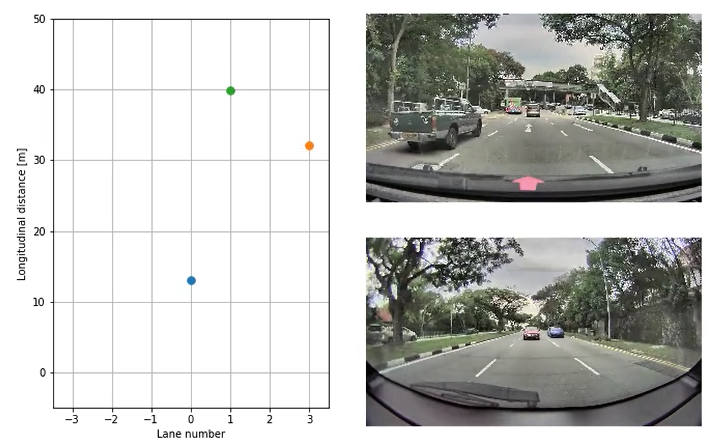
\includegraphics[width=0.8\linewidth]{bmw_example}
	\caption{Example of a frame of the data. In the left plot, the detected objects are shown (different color means different ID). On the right, the image of the front view camera (top) and rear view camera (bottom) are shown.}
	\label{fig:bmw example}
\end{figure}

\begin{itemize}
	\item I got access to a very small piece of the data acquired by BMW in Singapore. See \cref{fig:bmw example} for an example of a frame. Some observations:
	\begin{itemize}
		\item Many objects are not detected. For example, the car on the left side (see \cref{fig:bmw example}) is not detected. It seems that the field of view is very limited.
		\item The object data seems to be processed with a low pass filter with a very low bandwidth. For example, the car in front (see \cref{fig:bmw example}) already increased distance with approximately $\unit[5]{m}$, but this is only visible in the object data after few seconds.
	\end{itemize}
	\item I did some research regarding similarity measures for time series, because an appropriate similarity measure for comparing two different scenarios would be useful for at least two reasons:
	\begin{itemize}
		\item To quantify to what extent a certain set of scenario is complete, it would be useful to quantity the similarities among the scenarios. If each scenario is very different from all other scenarios, this is an indication that the set of scenarios does not reflect all possible variations. To quantify the `difference' between two scenarios, a (dis)similarity measure could be employed.
		\item To quantify how realistic a generated scenario is, it could be compared with real-world scenarios. If the generation scenarios differs significantly from generated scenarios, it could be an indication that the generation scenario is not realistic.
	\end{itemize}
	A report is attached to this progress report\footnote{Note that the page numbers in the table of contents are not correct, as those page numbers refer to the original report (before it was included in this progress report)} that reflects my findings.
	\item The paper for the Intelligent Vehicle Symposium (IV) 2018 is submitted. On the 31st of March we will receive a notification of acceptance. The paper is attached to this document (starting at page \pageref{ivpaper}).
\end{itemize}

\section{Future plans}

\begin{itemize}
	\item I wrote a document regarding similarity measures for time series. I want to apply one or several measures for quantifying the completeness of a set of real-world scenarios. I can use a small dataset with time series of the speed while the car is braking (approximately 3000 time series).
	\item For my work in Singapore, I need to define 15 different scenarios classes and the way we want to parametrize these scenarios. Ideally, I want to show at least one real-world scenario for each scenario class.
	\item 
\end{itemize}

\section{Questions}

\begin{itemize}
	\item 
\end{itemize}

\bibliographystyle{ieeetr}
\bibliography{../../bib}

\newpage
\includepdf[pages=-,pagecommand={},width=\paperwidth]{../../"20180207 Similarity"/scenario_similarity.pdf}
\label{ivpaper}
\includepdf[pages=-,pagecommand={},width=\paperwidth]{../../"20171111 IV2018 Ontology"/root.pdf}

\end{document}